\chapter{Les matières plastiques et les matériaux synthétiques}\label{ch:g8:plastics}

Compte les objets en plastique que tu touches en une matinée~: une
brosse à dents, une bouteille, un imperméable, une coque de téléphone,
le siège d'un bus, le sac des courses. Presque aucun n'existait il y a
cent vingt ans, et aucun n'a poussé sur un arbre ni n'a été extrait du
sous-sol. Les \omterm{def:g8:plastics:plastic}{matières plastiques} sont des matériaux inventés par les
chimistes --- légers, bon marché, imperméables, façonnables à volonté
--- et ce succès même est devenu un problème.

\begin{recall}
Les matériaux naturels s'utilisent à peu près tels qu'on les trouve dans
la nature~; les matériaux fabriqués sont obtenus en transformant des
\omterm{def:g5:raw-materials-and-recycling:raw-material}{matières premières}, et le \omterm{def:g5:raw-materials-and-recycling:recycling}{recyclage} transforme le matériau de vieux
objets en objets neufs (\cref{ch:g5:raw-materials-and-recycling}). La
\omterm{def:g4:what-a-fire-needs:burning}{combustion} d'un \omterm{def:g4:what-a-fire-needs:fuel}{combustible} fait de carbone et d'hydrogène donne du
dioxyde de carbone et de l'eau (\cref{ch:g8:combustion-and-fuels}).
\end{recall}

\begin{omfigure}
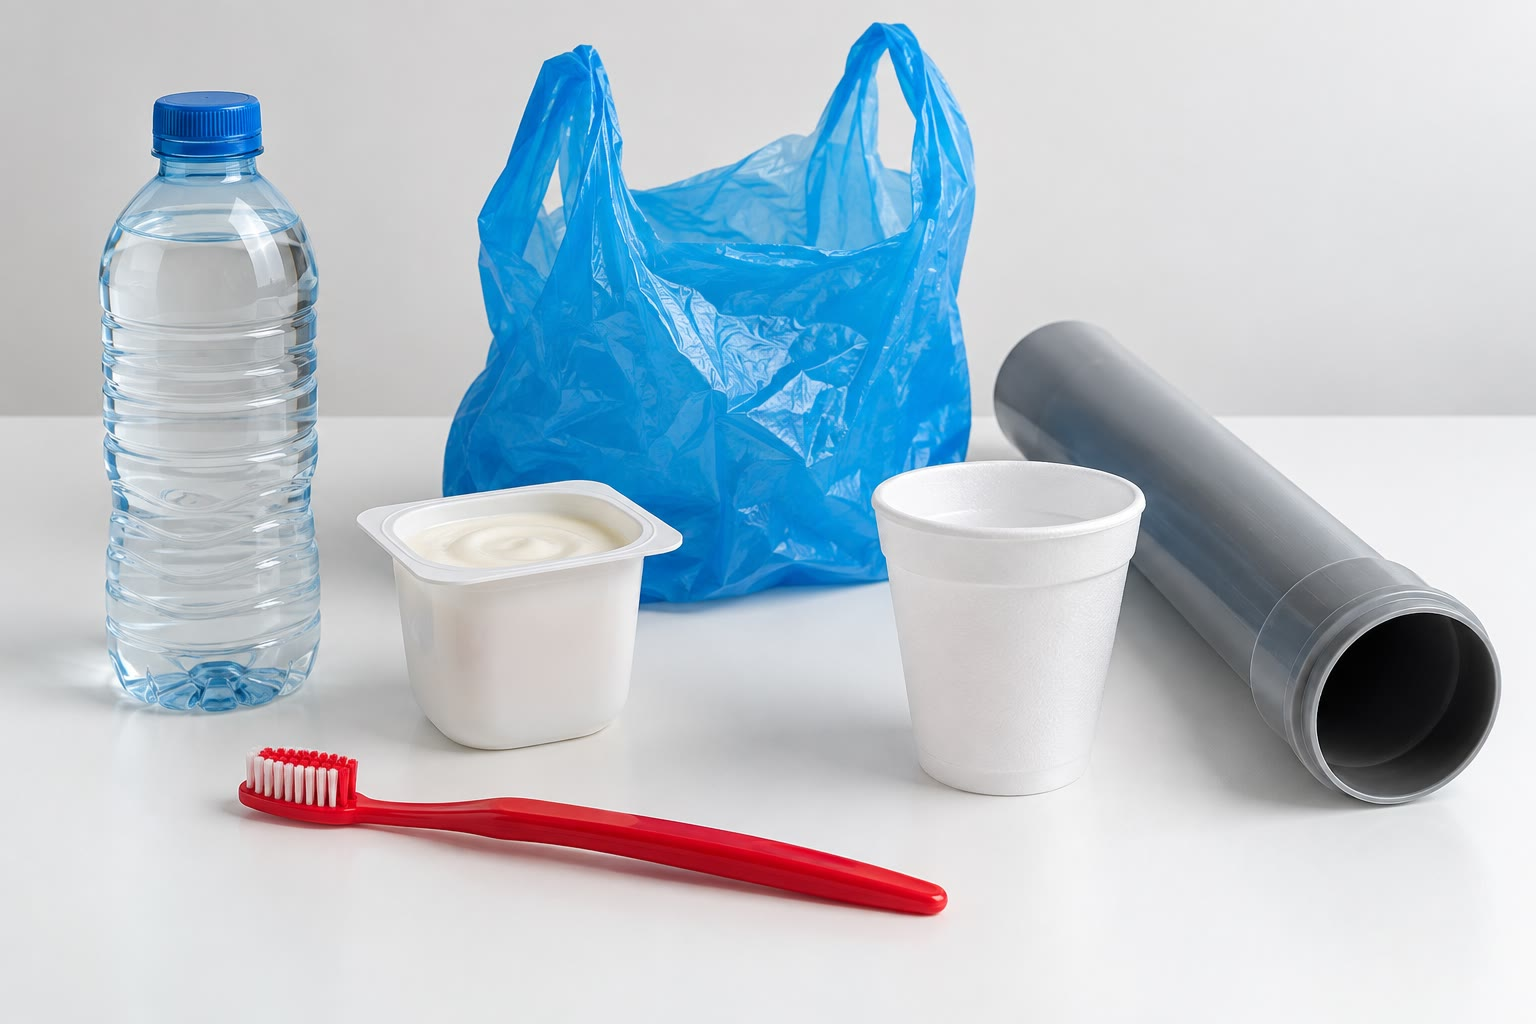
\includegraphics[width=0.55\linewidth]{images/book1/ai/g8-plastic-objects.jpg}

{\small Des objets en plastique de tous les jours~: une bouteille, un
pot, un sac, un tuyau, un gobelet, une brosse à dents.}
\end{omfigure}

\section{Matériaux naturels, artificiels et synthétiques}

\begin{definition}[Matériaux artificiels et synthétiques]\label{def:g8:plastics:artificial}
Parmi les matériaux fabriqués, un \emph{matériau
artificiel}\index{materiau artificiel@matériau artificiel} est obtenu en transformant
chimiquement un \omterm{def:g5:raw-materials-and-recycling:natural-material}{matériau naturel}~: le papier et la viscose (un tissu), à
partir de la cellulose du bois. Un \emph{matériau
synthétique}\index{materiau synthetique@matériau synthétique} est fabriqué à partir de
substances construites par les chimistes, le plus souvent à partir du
pétrole brut, et n'a pas d'équivalent naturel~: le nylon, le polyester,
les \omterm{def:g8:plastics:plastic}{matières plastiques}.
\end{definition}

\begin{omfigure}
\begin{tikzpicture}[font=\small, level distance=1.5cm,
    box/.style={draw=omDef, fill=omDef!6, rounded corners=2pt, align=center,
      inner sep=4pt, text width=3.3cm},
    level 1/.style={sibling distance=6.4cm},
    level 2/.style={sibling distance=3.8cm},
    edge from parent/.style={draw, thick, omDef, ->}]
  \node[box] {matériaux}
    child {node[box] {naturels\\ \footnotesize coton, laine, bois}}
    child {node[box] {fabriqués}
      child {node[box] {artificiels\\ \footnotesize papier, viscose}}
      child {node[box, draw=omProp, fill=omProp!6] {synthétiques\\ \footnotesize nylon,
        polyester, plastiques}}};
\end{tikzpicture}

{\small Matériaux naturels, artificiels et synthétiques.}
\end{omfigure}

\section{Ce que sont les matières plastiques}

\begin{definition}[Matière plastique]\label{def:g8:plastics:plastic}
Une \emph{matière plastique}\index{matiere plastique@matière plastique} est un \omterm{def:g8:plastics:artificial}{matériau
synthétique} fait de très longues \omterm{def:g7:atoms-and-molecules:molecule}{molécules}, que l'on peut mettre en
forme par moulage --- le plus souvent à chaud, quand elle est molle ---
et qui garde sa forme en refroidissant. La plupart des matières
plastiques sont fabriquées à partir de pétrole brut ou de gaz naturel.
\end{definition}

\begin{remark}[De très longues molécules]\label{rem:g8:plastics:long}
Une \omterm{def:g7:atoms-and-molecules:molecule}{molécule} d'eau contient trois \omterm{def:g7:atoms-and-molecules:atom}{atomes}~; une \omterm{def:g7:atoms-and-molecules:molecule}{molécule} de \omterm{def:g8:plastics:plastic}{matière
plastique} peut en contenir des dizaines de milliers, reliés en une
longue chaîne, comme un collier de perles identiques. La façon dont on
construit de telles chaînes est l'objet d'un chapitre de la fin de ce
livre.
\end{remark}

\begin{omfigure}
\begin{tikzpicture}[font=\small]
  \foreach \k in {0,...,17} {
    \pgfmathsetmacro\x{0.62*\k}
    \pgfmathsetmacro\y{0.35*sin(40*\k)}
    \shade[ball color=omDef!50] (\x,\y) circle (0.22);
  }
  \node[anchor=west] at (11.2,0) {\dots};
  \node[anchor=north, align=center] at (5.3,-0.6) {une chaîne de milliers de motifs identiques};
\end{tikzpicture}

{\small Une image, pas un modèle~: la \omterm{def:g7:atoms-and-molecules:molecule}{molécule} d'une \omterm{def:g8:plastics:plastic}{matière plastique}
est une très longue chaîne de motifs identiques.}
\end{omfigure}

\begin{history}[La bakélite, 1907]
La première \omterm{def:g8:plastics:plastic}{matière plastique} entièrement synthétique fut fabriquée par
le chimiste Leo Baekeland en 1907, à partir de phénol, tiré du goudron
de houille, et de formaldéhyde. Dure, sombre et résistante à la
chaleur, la bakélite devint le matériau des téléphones, des postes de
radio et des interrupteurs électriques. Le nylon suivit dans les années
1930, puis les plastiques des bouteilles et des sacs après la Seconde
Guerre mondiale.
\end{history}

\begin{omfigure}
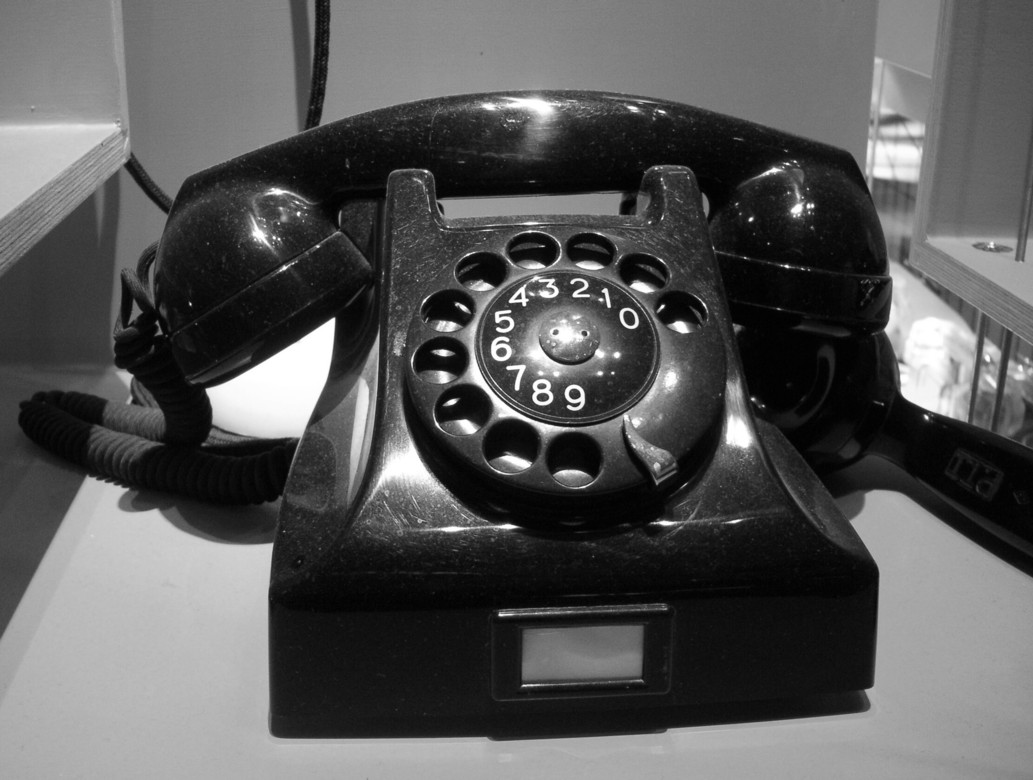
\includegraphics[width=0.42\linewidth]{images/book1/bakelite-telephone.jpg}

{\small Un téléphone en bakélite de 1947. Photo~: Holger Ellgaard,
CC BY-SA 3.0.}
\end{omfigure}

\section{Les principales matières plastiques et leurs codes}

\begin{definition}[Code d'identification des résines]\label{def:g8:plastics:code}
Le \emph{code d'identification des résines}\index{code d'identification des resines@code d'identification des résines}
est un nombre de 1 à 7, imprimé dans un triangle de flèches sur un objet
en plastique, qui désigne la \omterm{def:g8:plastics:plastic}{matière plastique} dont il est fait, afin
qu'on puisse le trier pour le \omterm{def:g5:raw-materials-and-recycling:recycling}{recyclage}. Le triangle ne signifie pas que
l'objet sera recyclé.
\end{definition}

\begin{proposition}[Sept codes]\label{prop:g8:plastics:codes}
Les codes, avec les usages les plus courants de chaque \omterm{def:g8:plastics:plastic}{matière
plastique}~:
\begin{center}
\small
\begin{tabular}{cll}
\hline
code & \omterm{def:g8:plastics:plastic}{matière plastique} & objets typiques \\
\hline
1 & PET, polytéréphtalate d'éthylène & bouteilles d'eau et de soda, fibres polaires \\
2 & PEHD, polyéthylène haute densité & bouteilles de lait et de shampooing, bouchons \\
3 & PVC, polychlorure de vinyle & tuyaux, cadres de fenêtres, câbles \\
4 & PEBD, polyéthylène basse densité & sacs, films \\
5 & PP, polypropylène & pots de yaourt, bouchons, pare-chocs \\
6 & PS, polystyrène & gobelets et barquettes en mousse, boîtiers de CD \\
7 & autres plastiques & \omterm{def:g6:pure-substances-and-mixtures:mixture}{mélanges}, emballages multicouches \\
\hline
\end{tabular}
\end{center}
\end{proposition}

\begin{omfigure}
\begin{tikzpicture}[font=\small]
  \foreach \n/\lab in {1/PET, 2/PEHD, 3/PVC, 4/PEBD, 5/PP, 6/PS, 7/AUTRES} {
    \begin{scope}[xshift=(\n-1)*2.1cm]
      \foreach \a in {90,210,330} {
        \pgfmathsetmacro\b{\a+120}
        \draw[omDef, line width=1.1pt, ->, >={Stealth[length=4pt]}]
          ($(\a:0.75)!0.14!(\b:0.75)$) -- ($(\a:0.75)!0.86!(\b:0.75)$);
      }
      \node[font=\bfseries] at (0,-0.05) {\n};
      \node[anchor=north, font=\footnotesize] at (0,-0.8) {\lab};
    \end{scope}
  }
\end{tikzpicture}

{\small Les sept \omterm{def:g8:plastics:code}{codes d'identification des résines}, chacun avec le nom
abrégé de sa \omterm{def:g8:plastics:plastic}{matière plastique}.}
\end{omfigure}

\section{Thermoplastiques et thermodurcissables}

\begin{definition}[Thermoplastique et thermodurcissable]\label{def:g8:plastics:thermoplastic}
Un \emph{thermoplastique}\index{thermoplastique} se ramollit chaque fois
qu'on le chauffe et durcit de nouveau en refroidissant~: on peut le
fondre et le mouler encore et encore (PET, polyéthylène, PVC,
polypropylène, polystyrène). Un
\emph{thermodurcissable}\index{thermodurcissable} durcit pour de bon la
première fois qu'on le chauffe et qu'on le moule~: chauffé de nouveau,
il ne se ramollit pas mais se carbonise (la bakélite, les résines des
colles et des coques de bateau).
\end{definition}

\begin{remark}[Lesquels se recyclent]\label{rem:g8:plastics:which}
Les \omterm{def:g8:plastics:thermoplastic}{thermoplastiques} peuvent être fondus et moulés de nouveau~: ce sont
les \omterm{def:g8:plastics:plastic}{matières plastiques} que l'on recycle en objets neufs. Les
\omterm{def:g8:plastics:thermoplastic}{thermodurcissables} ne peuvent pas être fondus de nouveau.
\end{remark}

\section{Les matières plastiques dans l'environnement}

\begin{proposition}[Les matières plastiques durent]\label{prop:g8:plastics:last}
% ledger: plastics:use-2019, plastics:waste-2019, plastics:recycled-share-2019
Le monde a utilisé environ 460 millions de tonnes de \omterm{def:g8:plastics:plastic}{matières plastiques}
en 2019 et jeté environ 353 millions de tonnes de déchets plastiques~;
le plastique recyclé ne représentait qu'environ \qty{6}{\percent} du
plastique utilisé. Les \omterm{def:g8:plastics:plastic}{matières plastiques} ne pourrissent pas~: dans la
nature, elles se brisent en morceaux de plus en plus petits, les
microplastiques, que l'on retrouve dans les rivières, les océans, les
sols et le corps des animaux.
\end{proposition}

\begin{omfigure}
\begin{minipage}[t]{0.48\linewidth}\centering
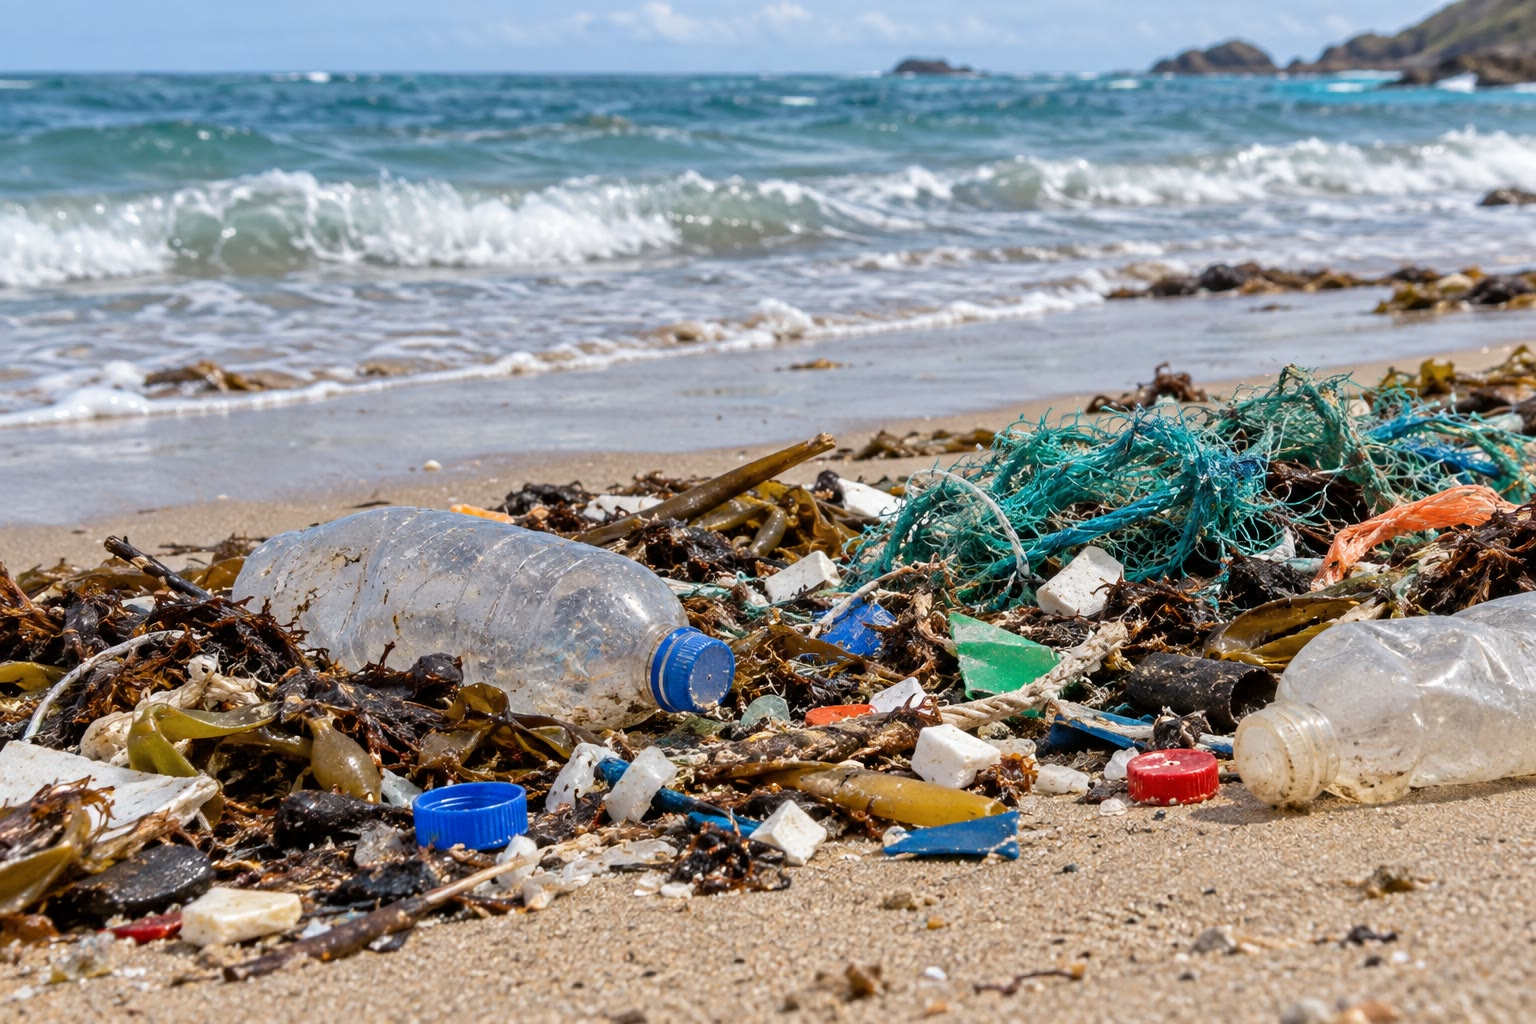
\includegraphics[width=\linewidth,height=4.6cm,keepaspectratio]{images/book1/ai/g8-beach-litter.jpg}

{\small Des déchets plastiques rejetés sur une plage.}
\end{minipage}\hfill
\begin{minipage}[t]{0.48\linewidth}\centering
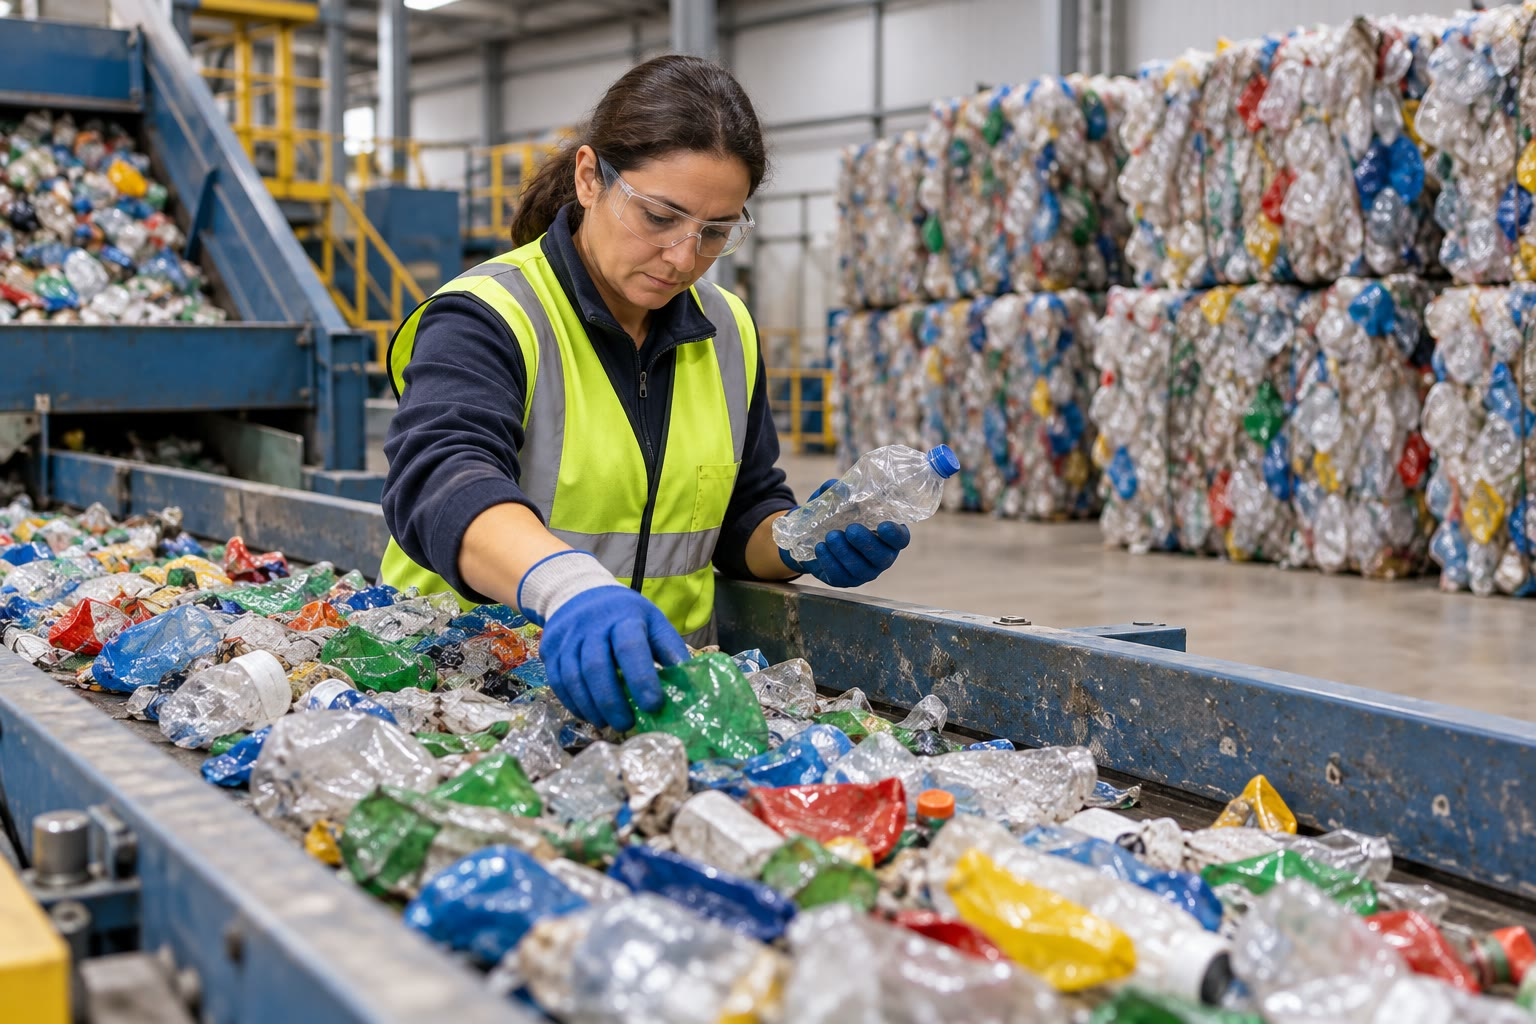
\includegraphics[width=\linewidth,height=4.6cm,keepaspectratio]{images/book1/ai/g8-sorting-line.jpg}

{\small Une chaîne de tri dans une usine de \omterm{def:g5:raw-materials-and-recycling:recycling}{recyclage} des plastiques.}
\end{minipage}
\end{omfigure}

\begin{remark}[Brûler les matières plastiques]\label{rem:g8:plastics:burning}
Les \omterm{def:g8:plastics:plastic}{matières plastiques} brûlent, et elles produisent du dioxyde de
carbone quand elles brûlent complètement. Mais brûlées dans un feu de
jardin, elles brûlent de façon incomplète et libèrent de la suie, du
monoxyde de carbone et d'autres substances nocives~; le PVC, qui
contient du chlore, dégage du chlorure d'hydrogène, un gaz corrosif. Les
déchets plastiques ne sont brûlés que dans des incinérateurs conçus
pour épurer leurs fumées.
\end{remark}

\section{Exercices}

\begin{exercise}[$\star$]\label{exo:g8:plastics:1}
Naturel, artificiel ou synthétique~? Le coton, le nylon, le papier, la
laine, le polystyrène, la viscose.
\end{exercise}

\begin{exercise}[$\star$]\label{exo:g8:plastics:2}
À partir de quelle \omterm{def:g5:raw-materials-and-recycling:raw-material}{matière première} la plupart des \omterm{def:g8:plastics:plastic}{matières plastiques}
sont-elles fabriquées~?
\end{exercise}

\begin{exercise}[$\star$]\label{exo:g8:plastics:3}
Quelle \omterm{def:g8:plastics:plastic}{matière plastique} porte le code 1~? Donne un objet fait de cette
matière.
\end{exercise}

\begin{exercise}[$\star$]\label{exo:g8:plastics:4}
Quelle est la différence entre un \omterm{def:g8:plastics:thermoplastic}{thermoplastique} et un
\omterm{def:g8:plastics:thermoplastic}{thermodurcissable}~?
\end{exercise}

\begin{exercise}[$\star\star$]\label{exo:g8:plastics:5}
Un pot de yaourt porte le code 5. Nomme sa \omterm{def:g8:plastics:plastic}{matière plastique}, et dis si
elle pourrait en principe être fondue et moulée de nouveau.
\end{exercise}

\begin{exercise}[$\star\star$]\label{exo:g8:plastics:6}
Pourquoi un triangle de flèches sur un objet ne signifie-t-il pas que
l'objet sera recyclé~?
\end{exercise}

\begin{exercise}[$\star\star$]\label{exo:g8:plastics:7}
Pourquoi le manche d'une poêle est-il souvent fait d'un \omterm{def:g8:plastics:thermoplastic}{thermodurcissable}
plutôt que d'un \omterm{def:g8:plastics:thermoplastic}{thermoplastique}~?
\end{exercise}

\begin{exercise}[$\star\star$]\label{exo:g8:plastics:8}
D'après les chiffres de ce chapitre pour 2019, quel pourcentage du
plastique utilisé est devenu un déchet cette année-là~? Arrondis à
l'unité.
\end{exercise}

\begin{exercise}[$\star\star$]\label{exo:g8:plastics:9}
Pourquoi ne faut-il jamais \omterm{def:g4:what-a-fire-needs:burning}{brûler} du PVC dans un feu de jardin~?
\end{exercise}

\begin{exercise}[$\star\star$]\label{exo:g8:plastics:10}
Une école utilise 300 bouteilles de \qty{25}{g} chacune par semaine,
pendant 36 semaines de l'année. Quelle masse de plastique cela
représente-t-il en un an~?
\end{exercise}

\begin{exercise}[$\star\star\star$]\label{exo:g8:plastics:11}
Le polyéthylène n'est fait que de carbone et d'hydrogène. Écris les
produits de sa \omterm{def:g8:combustion-and-fuels:complete}{combustion complète}. Explique pourquoi le \omterm{def:g4:what-a-fire-needs:burning}{brûler} ajoute du
dioxyde de carbone à l'\omterm{def:g4:air-a-mixture-of-gases:air}{air}, comme un \omterm{def:g8:combustion-and-fuels:fossil}{combustible fossile}.
\end{exercise}

\begin{exercise}[$\star\star\star$]\label{exo:g8:plastics:12}
Explique comment une bouteille en plastique perdue en mer peut finir,
des années plus tard, sous forme de microplastiques dans un poisson.
\end{exercise}

\section{Problème~: la chaîne de tri}

\begin{problem}[{Problème du week-end --- une tonne de bouteilles usagées,
leurs codes, et les paillettes de plastique propres qui sortent de
l'usine}]
\label{pb:g8:plastics:1}
Une usine de \omterm{def:g5:raw-materials-and-recycling:recycling}{recyclage} reçoit des balles de bouteilles de boisson
usagées. Une balle typique de \qty{1}{t} (\qty{1000}{kg}) contient, en
masse~: \qty{80}{\percent} de corps de bouteilles en PET,
\qty{12}{\percent} de bouchons (PEHD et PP), \qty{5}{\percent}
d'étiquettes (film de PP) et \qty{3}{\percent} de saletés et de restes
de liquide. Des machines séparent les bouchons et les étiquettes des
corps, le PET est broyé en paillettes, et les paillettes sont lavées~;
le lavage fait perdre \qty{2.5}{\percent} du PET. Les paillettes
propres sont fondues et filées en fibres pour des vestes polaires.

\medskip
\noindent\textbf{Partie I --- Les \omterm{def:g8:plastics:plastic}{matières plastiques}.}
\begin{enumerate}
  \item Quel code est imprimé sur les corps des bouteilles~? Sur les
        bouchons~?
  \item Ces \omterm{def:g8:plastics:plastic}{matières plastiques} sont-elles naturelles, artificielles ou
        synthétiques~?
  \item Peut-on fondre et filer de nouveau le PET~? Quelle sorte de
        \omterm{def:g8:plastics:plastic}{matière plastique} est-ce donc~?
  \item Pourquoi sépare-t-on les bouchons et les étiquettes des corps
        avant de fondre le PET~?
\end{enumerate}

\medskip
\noindent\textbf{Partie II --- La balle.}
\begin{enumerate}[resume]
  \item Quelle masse de PET une balle contient-elle~?
  \item Quelle masse de bouchons~? D'étiquettes~?
  \item Quelle masse de la balle n'est pas du plastique~?
  \item Quel pourcentage de la balle est du plastique~?
\end{enumerate}

\medskip
\noindent\textbf{Partie III --- Les paillettes.}
\begin{enumerate}[resume]
  \item Quelle masse de PET est perdue au lavage~?
  \item Une veste polaire demande \qty{0.39}{kg} de fibre de PET. Pourquoi
        vaut-il mieux la fabriquer à partir de paillettes qu'à partir de
        PET neuf~?
  \item L'usine pourrait \omterm{def:g4:what-a-fire-needs:burning}{brûler} les bouchons et les étiquettes pour
        produire de la chaleur au lieu de les recycler. Nomme le gaz que
        cela ajouterait à l'\omterm{def:g4:air-a-mixture-of-gases:air}{air}.
  \item Calcule la masse de paillettes de PET propres que fournit une
        balle.
\end{enumerate}
\end{problem}
